\chapter{Frontier and Scale Boundary}
\label{chap:frontier}

\section{Within-Family Scaling: Does the Gap Grow with Capability?}

Before turning to hosted frontier models, we ask a sharper question inside one model family: as a Qwen model gets larger, does the Banglish gap shrink (capability helps) or grow (capability is spent on the easier scripts)? We run the frozen validation-200 v5 triad on four additional Qwen sizes --- Qwen2.5-0.5B and 1.5B, and Qwen3-0.6B and 1.7B (no-thinking) --- and combine them with the three thesis-facing models on the same frozen slice.

\begin{table}[H]
\centering
\caption{Within-family Qwen scaling on validation-200 v5. Gap is reviewed Banglish minus Bangla, with paired bootstrap 95\% CI and McNemar exact p.}
\label{tab:scaling}
\small
\begin{tabular}{llrrrll}
\hline
Model & Family & Params (B) & Bangla & Banglish & Gap (pts) & McNemar $p$ \\
\hline
Qwen2.5-0.5B & Qwen2.5 & 0.49 & 40/200 & 46/200 & +3.0, CI [-1.5, +7.5] & 0.263 \\
Qwen2.5-1.5B & Qwen2.5 & 1.54 & 46/200 & 40/200 & -3.0, CI [-9.0, +3.0] & 0.418 \\
Qwen2.5-3B & Qwen2.5 & 3.09 & 54/200 & 41/200 & -6.5, CI [-13.0, 0.0] & 0.066 \\
Qwen2.5-7B 8-bit & Qwen2.5 & 7.62 & 65/200 & 47/200 & -9.0, CI [-16.5, -1.5] & 0.022 \\
Qwen3-0.6B & Qwen3 & 0.60 & 35/200 & 29/200 & -3.0, CI [-8.0, +2.0] & 0.345 \\
Qwen3-1.7B & Qwen3 & 1.72 & 33/200 & 35/200 & +1.0, CI [-5.5, +7.5] & 0.878 \\
Qwen3-4B & Qwen3 & 4.02 & 80/200 & 49/200 & -15.5, CI [-22.0, -9.0] & $<$0.0001 \\
\hline
\end{tabular}%
\end{table}

\begin{figure}[H]
\centering
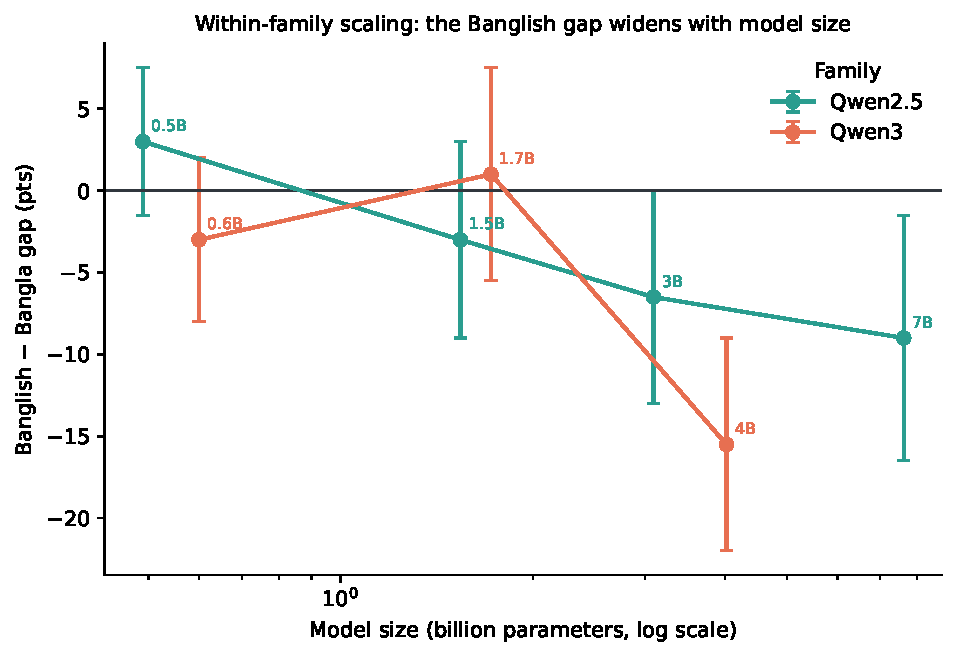
\includegraphics[width=0.82\textwidth]{figures/fig_scaling_curve.pdf}
\caption{Banglish minus Bangla gap versus model size within the Qwen2.5 and Qwen3 families on validation-200 v5, with paired bootstrap 95\% confidence intervals.}
\label{fig:scaling}
\end{figure}

The Qwen2.5 family shows a clean monotonic trend: the gap moves from $+3.0$ points at 0.5B (where the model is too weak for the contrast to mean much) through $-3.0$, $-6.5$, and $-9.0$ points at 1.5B, 3B, and 7B, and the McNemar p-value falls correspondingly from 0.26 to 0.02. The gap does not close with capability; it widens. The Qwen3 family is noisier at the bottom --- the 1.7B no-thinking point is weak and near zero --- but its largest model has by far the largest gap ($-15.5$ points, $p < 0.0001$). The reading is consistent with the thesis mechanism: added capability is preferentially spent on the higher-resource Bangla and English views, so the romanized-script deficit persists or grows rather than being absorbed. This makes the script gap a property that scaling alone, within these compact families, does not fix.

\section{Frontier API Boundary}

The frontier/API panel tests whether the gap disappears for stronger or hosted models. The answer is not a simple yes or no. Stronger models can reduce the gap, but the reduction is uneven and model-dependent.

\begin{table}[H]
\centering
\caption{Validation-200 v5 frontier/API panel. Difference columns report reviewed Banglish minus the comparison script.}
\label{tab:api-panel}
\small
\resizebox{\textwidth}{!}{%
\begin{tabular}{lllllll}
\hline
Model & Score & Bangla & Reviewed Banglish & English & Banglish--Bangla & Banglish--English \\
\hline
Gemini 3.5 Flash & Strict & 163/200 & 136/200 & 144/200 & -13.5 pts & -4.0 pts \\
Gemini 3.5 Flash & Secondary & 170/200 & 161/200 & 165/200 & -4.5 pts & -2.0 pts \\
GPT-5.5 low & Strict & 172/200 & 169/200 & 154/200 & -1.5 pts & +7.5 pts \\
GPT-5.5 low & Secondary & 173/200 & 174/200 & 168/200 & +0.5 pts & +3.0 pts \\
Claude Sonnet 4.6 & Strict & 162/200 & 130/200 & 153/200 & -16.0 pts & -11.5 pts \\
Claude Sonnet 4.6 & Secondary & 167/200 & 133/200 & 166/200 & -17.0 pts & -16.5 pts \\
DeepSeek V4 Flash & Strict & 143/200 & 82/200 & 132/200 & -30.5 pts & -25.0 pts \\
DeepSeek V4 Flash & Secondary & 152/200 & 96/200 & 148/200 & -28.0 pts & -26.0 pts \\
Groq Llama 3.3 70B & Strict & 90/200 & 48/200 & 102/200 & -21.0 pts & -27.0 pts \\
Groq Llama 3.3 70B & Secondary & 92/200 & 56/200 & 111/200 & -18.0 pts & -27.5 pts \\
\hline
\end{tabular}%
}
\end{table}

GPT-5.5 low is the strongest boundary case. Under strict scoring it nearly closes the Banglish-vs-Bangla gap: 172/200 Bangla versus 169/200 Banglish. Under secondary scoring, Banglish is slightly ahead of Bangla. This is an important limitation on the main claim. With enough capability and answer recovery, the reviewed-Banglish gap can nearly disappear on the validation-200 set.

The McNemar exact tests make the panel contrast precise. GPT-5.5's strict Bangla-versus-Banglish discordance is 6 losses against 3 gains ($p = 0.51$): statistically indistinguishable from no gap. Every other API row is significant after Holm correction across the panel ($p < 0.0001$ for Gemini, Claude, DeepSeek, and Groq under strict scoring), with conditional odds ratios from 3.9 (Groq) to 9.1 (DeepSeek). The full per-panel tables are in \url{https://github.com/munimthahmid/BanglishBench/blob/main/reports/mcnemar_script_gaps.md}.

But that is not the whole frontier story. Gemini 3.5 Flash reduces the gap but retains a strict deficit. Claude Sonnet 4.6 has high absolute accuracy but still scores 32 items lower on reviewed Banglish than on Bangla under strict scoring. It also produces more long and multiline answers under an answer-only prompt, which creates format-compliance and cost issues. DeepSeek V4 Flash and Groq-hosted Llama 3.3 70B retain large Banglish deficits.

The correct conclusion is therefore not ``frontier models solve Banglish.'' It is more precise: stronger models can reduce the semantic gap, but script robustness remains model-dependent, parser-dependent, and cost-dependent.

\section{BEnQA Scale Extension}

The validation-200 reviewed core is deliberately small and carefully audited. That is a strength for controlled analysis, but it also raises an obvious scale question: does the pattern survive beyond the selected 200 items? We answer that with a larger BEnQA-only human-reviewed extension.

The extension construction starts from 4,939 eligible BEnQA source rows after excluding the frozen gold-core BEnQA items. We select 1,000 rows with deterministic subject-balanced sampling. The human review audit accepts 618 rows unchanged, edits 356 rows, and rejects 26 rows. The 974 accepted or edited rows form the BEnQA human-reviewed gold extension used for large-scale evaluation.

This extension does not replace validation-200 v5 because it is BEnQA-only and therefore covers science multiple-choice questions rather than the mixed BEnQA-plus-BanglaMATH task design. Its role is scale: combined with the validation core, the thesis now has 1,174 usable human-reviewed paired items, while preserving the 200-item core as the mixed-task primary benchmark.

\begin{table}[H]
\centering
\caption{BEnQA human-reviewed gold 974 scale results. The final column reports the Holm-adjusted McNemar exact p-value for the Bangla-versus-Banglish contrast.}
\label{tab:ext974}
\small
\resizebox{\textwidth}{!}{%
\begin{tabular}{lllllll}
\hline
Model & Bangla & Reviewed Banglish & English & Banglish--Bangla & Banglish--English & McNemar $p$ \\
\hline
Qwen2.5-3B & 323/974 & 285/974 & 490/974 & -3.90 pts, CI [-7.19, -0.51] & -21.05 pts, CI [-24.64, -17.35] & 0.024 \\
Gemini 3.5 Flash & 743/974 & 633/974 & 680/974 & -11.29 pts, CI [-13.66, -8.93] & -4.83 pts, CI [-7.39, -2.05] & $<$0.0001 \\
GPT-5.5 none & 820/974 & 699/974 & 825/974 & -12.42 pts, CI [-15.09, -9.75] & -12.94 pts, CI [-15.91, -9.86] & $<$0.0001 \\
Claude Sonnet 4.6 & 764/974 & 524/974 & 771/974 & -24.64 pts, CI [-27.82, -21.25] & -25.36 pts, CI [-28.64, -21.87] & $<$0.0001 \\
DeepSeek V4 Flash & 756/974 & 438/974 & 791/974 & -32.65 pts, CI [-36.04, -29.26] & -36.24 pts, CI [-39.73, -32.96] & $<$0.0001 \\
Groq Llama 3.3 70B & 547/974 & 333/974 & 622/974 & -21.97 pts, CI [-25.67, -18.17] & -29.67 pts, CI [-33.26, -26.08] & $<$0.0001 \\
\hline
\end{tabular}%
}
\end{table}

All six 974-row extension runs reproduce the same core pattern: \textbf{reviewed Banglish is the weakest script view for every model}, with every Bangla-versus-Banglish contrast significant under the Holm-corrected McNemar exact test. The compact open model and the Groq, DeepSeek, and GPT-5.5 rows additionally show the full English \textgreater{} Bangla \textgreater{} reviewed Banglish ordering; Gemini is the one model whose Bangla accuracy exceeds its English accuracy, which does not change the Banglish conclusion.

The most consequential row is GPT-5.5. On validation-200 it nearly closes the gap; on the 974-row extension, run with no reasoning effort, it loses 12.42 points on reviewed Banglish relative to Bangla ($p < 0.0001$). The near-closure observed on the 200-item core therefore does not generalize to the larger slice under a low-compute configuration. Script robustness at the frontier is not a solved property; it depends on the model, the reasoning budget, and the evaluation scale.

The models behave differently in absolute accuracy. DeepSeek V4 Flash is far stronger than Qwen2.5-3B on the extension. But the Banglish deficit remains, and for DeepSeek it is much larger. This is one of the strongest results in the thesis. It shows that higher absolute accuracy does not guarantee Banglish robustness, and that the extension result is not a Qwen-local artifact. One operational caveat: the Gemini extension run has elevated parsed-empty counts (176--263 rows per variant), so its absolute scores are less clean than its paired contrast.

The 974-row runs also provide qualitative examples. Qwen2.5-3B has 346 recoverable reviewed-Banglish misses, Groq-hosted Llama 3.3 70B has 406, DeepSeek V4 Flash has 424, Claude Sonnet 4.6 has 330, GPT-5.5 has 199, and Gemini 3.5 Flash has 166. These are cases where reviewed Banglish is wrong but Bangla or English is correct on the same item. They are useful for error analysis and defense slides, but they are not a separate statistical test.

\subsection{Where the extension gap concentrates: subject breakdown}

The 974-row extension is large enough to split by macro subject (Biology 229, Physics 226, Math 223, Chemistry 221, Science 75 items). Table~\ref{tab:ext-subjects} reports the Banglish-minus-Bangla gap per subject.

\begin{table}[H]
\centering
\caption{BEnQA human-gold 974 extension: reviewed Banglish minus Bangla gap in points by macro subject. Stars mark within-subject McNemar exact $p<0.05$.}
\label{tab:ext-subjects}
\small
\resizebox{\textwidth}{!}{%
\begin{tabular}{lrrrrr}
\hline
Model & Biology & Chemistry & Physics & Math & Science \\
\hline
Qwen2.5-3B & -3.1 & -5.4 & -6.6 & -2.7 & +2.7 \\
Gemini 3.5 Flash & -13.1* & -14.5* & -10.2* & -10.8* & -1.3 \\
GPT-5.5 none & -17.9* & -14.9* & -13.3* & -3.6 & -12.0* \\
Claude Sonnet 4.6 & -33.2* & -25.8* & -30.1* & -6.3* & -33.3* \\
DeepSeek V4 Flash & -38.0* & -39.4* & -37.2* & -13.5* & -40.0* \\
Groq Llama 3.3 70B & -26.2* & -24.0* & -24.3* & -9.9* & -32.0* \\
\hline
\end{tabular}%
}

\smallskip
{\footnotesize Full per-subject accuracy and discordant-pair tables: \url{https://github.com/munimthahmid/BanglishBench/blob/main/reports/benqa_human_gold_974_subject_breakdown.md}.}
\end{table}

The breakdown reveals a consistent structure. For every frontier model, the Banglish gap is smallest on Math and largest on the text-heavy science subjects, with Biology and Science often worst. GPT-5.5's Math gap is statistically indistinguishable from zero ($-3.6$ points, $p = 0.28$) while its Biology gap is $-17.9$ points ($p < 0.0001$). DeepSeek loses around 38--40 points on the science subjects but 13.5 on Math. The pattern matches the mechanism the thesis proposes: romanization damages lexical grounding of Bangla terminology, and items whose content survives in symbolic or numeric form are less exposed. The script gap is therefore not uniform difficulty inflation; it concentrates where the question depends on reading romanized Bangla words.

\section{Natural Code-Mixed External Layer}

The controlled benchmark uses curriculum-style QA and math. That gives strong paired evidence, but it does not fully represent natural social media Banglish. We therefore add a separate ecological-validity layer using BnSentMix, a Bengali-English code-mixed sentiment dataset \cite{bnsentmix2024}.

We build a balanced 200-row four-way sentiment slice with 50 positive, 50 negative, 50 neutral, and 50 mixed items. The task is not paired by script, so it cannot estimate a Bangla-vs-Banglish script penalty. It answers a different question: do compact open models handle naturally occurring Bengali-English mixed text reliably?

\begin{table}[H]
\centering
\caption{BnSentMix natural code-mixed sentiment results}
\label{tab:bnsentmix}
\small
\begin{tabular}{llll}
\hline
Model & Accuracy & Macro-F1 & Valid outputs \\
\hline
Qwen2.5-3B & 89/200 & 0.431 & 200/200 \\
Qwen2.5-7B 8-bit & 98/200 & 0.479 & 200/200 \\
Qwen3-4B & 99/200 & 0.486 & 200/200 \\
\hline
\end{tabular}%
\end{table}

The models are above the 25\% majority baseline, but absolute accuracy remains modest. The error-overlap analysis shows substantial complementarity: the best single model is 99/200, while a diagnostic any-model oracle reaches 154/200. This oracle is not deployable because it chooses the correct model after seeing the gold label. Its value is diagnostic: model errors on natural code-mixed text are not uniform.

This layer supports the broader motivation that Bengali-English mixed text is difficult and user-relevant. It does not replace the controlled paired script-gap result.

\endinput
